The next method returns to the idea of water contact angles on metal surfaces. As described previously, water will spread completely on a nearly-flat metal surface surrounded by a gaseous environment. Instead of a gaseous environment, the water-metal system can be surrounded by another liquid. It has been observed that instead of wetting completely, a water droplet will only partially wet a metal when the surrounding environment is an immiscible liquid. This is called the two-liquid-phase contact angle method developed by Jacques Schultz.\cite{Schultz1977,Schultz1977a,Schultz1992} 

A full derivation of this method can be found in Appendix \ref{appendixB}. In order to calculate the dispersive component of \gamSV for a solid surface, the water \ca must be measured on a solid immersed in \nalk[s]. By interpreting Equation \ref{schultz2} as a classic linear function, $y = mx + b$:

\[
\underbracket{\gamma_{W}-\gamma_{H}+\gamma_{WH}\cos\theta_{W}}_{\text{\normalsize{$y$}}} =
\underbracket{2(\gamma_{S}^{D})^{1/2}}_{\text{\normalsize{$m$}}}  
\underbracket{[(\gamma_{W}^{D})^{1/2}-(\gamma_{H}^{D})^{1/2}] }_{\text{\normalsize{$x$}}} + 
\underbracket{I_{SW}^{P}}_{\text{\normalsize{$b$}}} 
\] 
$\gamma_{W}$, $\gamma_{H}$, and $\gamma_{WH}$ are known from consistently confirmed literature values,\cite{Chassin1986,Smitthipong2004,Takanashi2013,Nakamura2015} and are listed in Table \ref{knownsurften}. A data set of \textit{xy}-coordinates will be made by dropping water in an \nalk environment to determine $\gamma_{S}^{D}$ and $I_{SW}^{P} $. $\gamma_{S}^{D} $ will be calculated from the slope of the measured dataset. 

\begin{table}[h!]
	\centering
	\caption{Hydrocarbon surface tension and water-hydrocarbon interfacial energy}
	\begin{tabular} { |c||c|c|  } %\label{nalkSE}
		%	\hline
		%	\multicolumn{3}{|c|}{Hydrocarbon surface tension and water-hydrocarbon interfacial energy}\\
		\hline
		\textbf{\nalk[s]}	&\textbf{$\bm{\gamma_{H}}$ (mJ/m$\bm{^{2}}$)}	&\textbf{$\bm{\gamma_{WH}}$ (mJ/m$\bm{^{2}}$)}	\\
		\hline
		hexane		&18.4	&50.1 \\
		\hline
		octane		&21.7	&49.8 \\
		\hline
		decane		&23.8	&51.0 \\
		\hline
		hexadecane	&27.5	&51.3 \\
		\hline
	\end{tabular}
	\label{knownsurften}
\end{table}

%TODO: define London 

The polar component of the solid surface energy is determined using the same method described above,\cite{Schultz1977} but the bulk liquids now have both dispersive and polar components. This is also derived in Appendix \ref{appendixB}. These bulk liquids of chloroalkanes, nitroalkanes, aromatics, or alcohols are expected to establish a linear relationship between $I_{SW}^{P} $ and the square root of the polar component of surface tension from the bulk liquids. Schultz \etal suggests that this result allows all nondispersive interactions to be grouped together as a polar interaction, and they may be represented by the geometric mean of the polar component of the surface free energy of liquid and solid, as proposed by Owens and Wendt in Equation \ref{Isw}. This expression is verified experimentally, but there are no theoretical reasons why all nondispersive interactions should be represented by a geometric-mean expression.\cite{Fowkes1964}

\begin{equation}
\label{Isw}
	\begin{split}
	I_{SW}^{P} 							& = 2 (\gamma_{S}^{P}\gamma_{L}^{P})^{1/2} \\
	\rightarrow ~ \gamma_{S}^{P}	& = \frac{(I_{SW}^{P})^{2} }{4\gamma_{L}^{P}} 
	\end{split}
\end{equation}
The solid surface energy can then be determined from Equation \ref{gamS}:
\begin{equation}
\label{gamS}	\gamma_{S} = \gamma_{S}^{D} + \gamma_{S}^{P}	
\end{equation}



\subsection{Preliminary investigation of Cleaved Mica}
Preliminary two-liquid-phase method experiments on muscovite mica showed quick and complete wetting of water on pristine mica surfaces cleaved in decane and hexadecane, contradictory to published results.\cite{Schultz1992} Clearly, more iterations of this experiment must be done to recreate this seminal paper's data, but this made me consider how a water droplet on a mirror-finished material of even greater surface energy (e.g. Fe and Fe alloys) would spread even faster than it had on a pristine mica surface. A \ca may not stabilize on a well-polished Galfenol sample even using this two-liquid-phase method, thus we must consider more options to create a measurable \ca that can extract Young's \ca. 

When mica samples were removed from the decane environment, they were wiped clean with lint-free wipes and further cleaned with acetone. When the samples were returned to the decane environment, a droplet wet the surface with an observable \ca. When this process was repeated in hexadecane, the observed \ca increased as observed in Schultz \etal This shows that even a rough surface can be measured for surface energy using the two-liquid-phase method. 

%TODO Insert images from the cleaved mica experiments to show this progression

If this roughness is controlled by patterning the surface to a specific geometry, the same trend can be observed with the added benefit of a robust calculation of Young's contact angle by way of Equation \ref{cassie_coplanar}. 


\begin{equation}
\label{cassie_gen}	
\cos\theta_{CB} = f_{1}\cos\theta_{Y} - f_{2}
\end{equation}
\begin{equation}
\label{cassie_coplanar}	
\cos\theta_{CB} = f\cos\theta_{Y} - (1-f)
\end{equation}




\subsection{Beyond flat surface Schultz Method}
Since Schultz published his seminal paper, his method has been used to measure very high surface energy materials ranging from ~50 mJ/m$^{2}$ to 487 mJ/m$^{2}$.\cite{Nakamura2015} However, many of these studies fail to consider the wetting modes of water on their solid surfaces in a bulk \nalk environment. Giljean \etal examines the dependence of contact angles on the roughness of high surface energy titanium surfaces using the two-liquid-phase method. They show that, depending on the cleaning technique used to remove surface contaminations, the contact angle will change more with a decrease in roughness. Sound arguments are made for the type of wetting regime (Wenzel, Cassie-Baxter, or somewhere in-between) encountered at each step of wetting. An issue occurs when the authors attempt to use the Cassie-Baxter equation to calculate the Young \ca. The Cassie-Baxter equation (Equation \ref{cassie_gen}), as defined in the original publication,\cite{Cassie1944} is designed for a general surface, where $f_1$ is the \textit{total} area of solid under the drop per unit projected area under the drop and $\theta_Y,1$ is the contact angle on a smooth surface of material 1. $f_2$ is defined similarly to $f_2$ where material 2 is air or some other medium. Many papers, as pointed out by Milne \etal,\cite{Milne2012} falsely use Equation \ref{cassie_coplanar} for randomly rough surfaces when this equation is for the special case of a coplanar liquid-vapor and solid-liquid interface, as illustrated in Figure \ref{fig:cassie_coplanar}. To use this simple equation, a surface would have to be patterned with rectangular pillars with a small enough spacing to prevent capillary forces from causing the liquid to penetrate the roughness. 

%Keeping this in mind, I moved to the two-liquid-phase experiment originally performed on cleaved mica sheets. 



Considering all these factors, I postulate that by combining the two-liquid-phase method with a patterned surface of single-crystal Galfenol, the probe water droplet will not spread and a Young's \ca can be calculated for use in measuring the orientation-dependent surface energy of Galfenol. Single-crystal Galfenol samples were prepared at the DOE Ames Laboratory by the modified Bridgman technique at compositions of \fegacomp where $x=19,25$. These samples can be cut to obtain target orientations \hkl(100), \hkl(110), and \hkl(111) using electro-discharge machining. The isotropic surface created by single-crystal samples ensure that the triple-phase-line will maintain exactly the same $L_1-S$ interaction about the entire droplet perimeter. The patterned surfaces will be etched to have large enough pillars which retain as much surface orientation dependence on the contact angle as possible, as well as small enough gaps to allow for a Cassie-Baxter state in the $ L_1-L_2-S $ system. A Cassie-Baxter wetting mode would offer the greatest \ca of the three main wetting modes illustrated in Figure \ref{fig:young_cassie_wenzel}, and if a well patterned surface can be achieved similar to Figure \ref{fig:cassie_coplanar}, the Young \ca can be easily calculated from Equation \ref{cassie_coplanar}. 


\begin{figure}[h]
	\centering
	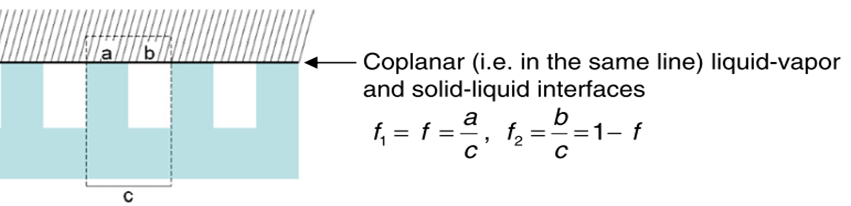
\includegraphics[width=0.7\linewidth]{cassie_coplanar}
	\caption{Schematic close up of three rough 2-D surfaces. Solid is blue/gray, air is white, liquid is the cross-hatched area above the surface. Liquid–vapor and solid–liquid interfaces of drop are denoted by the black line. A smooth-topped rough surface, which (for zero penetration of liquid) has coplanar solid–liquid and liquid–vapor interface (i.e. interfaces are in line with each other). This yields $ f_{1}=f $ and $ f_{2}=(1-f) $. Image source: \cite{Milne2012}}
	\label{fig:cassie_coplanar}
\end{figure}

\begin{figure}[h]
	\centering
	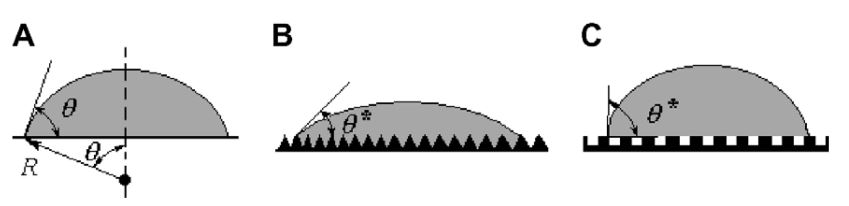
\includegraphics[width=\linewidth]{young_cassie_wenzel}
	\caption{Schemes of different wetting regimes. A – flat substrate; B – rough substrate, the Wenzel regime; C – rough substrate with air trapped under the drop, the Cassie–Baxter regime.\cite{Whyman2008}}
	\label{fig:young_cassie_wenzel}
\end{figure}

\subsection{Modeling surface geometry for Cassie-Baxter favoribility}

%TODO include modelling for surface geometries that will guarantee a Cassie-Baxter state and how CB angles transfer to flat surface angles. 

\subsection{Predicted errors in experiment}
Possible errors with this method will arise from non-atomically flat surfaces and pillars, imperfect Cassie-Baxter states caused by gravity or capillary forces drawing the probe liquid into the gaps between pillars, and oxide formation at the sample surface. However, such errors should be neglible given extensive polishing protocol, the immiscibility of water with \nalk[s], a controlled surface patterning, and a known cleaning procedure for rough metal surfaces. Therefore, I propose the assumption that our $ L_1-L_2-S $ system can be treated as the coplanar state depicted in Figure \ref{fig:cassie_coplanar} is reasonable. Concerning the displacement of \nalk[s] by water during the droplet depositing step, the wetting criteria has been proven by Schultz \etal\cite{Schultz1992,Giljean2011}. 
